% Options for packages loaded elsewhere
\PassOptionsToPackage{unicode}{hyperref}
\PassOptionsToPackage{hyphens}{url}
\PassOptionsToPackage{dvipsnames,svgnames,x11names}{xcolor}
%
\documentclass[
  letterpaper,
  DIV=11,
  numbers=noendperiod]{scrartcl}

\usepackage{amsmath,amssymb}
\usepackage{iftex}
\ifPDFTeX
  \usepackage[T1]{fontenc}
  \usepackage[utf8]{inputenc}
  \usepackage{textcomp} % provide euro and other symbols
\else % if luatex or xetex
  \usepackage{unicode-math}
  \defaultfontfeatures{Scale=MatchLowercase}
  \defaultfontfeatures[\rmfamily]{Ligatures=TeX,Scale=1}
\fi
\usepackage{lmodern}
\ifPDFTeX\else  
    % xetex/luatex font selection
\fi
% Use upquote if available, for straight quotes in verbatim environments
\IfFileExists{upquote.sty}{\usepackage{upquote}}{}
\IfFileExists{microtype.sty}{% use microtype if available
  \usepackage[]{microtype}
  \UseMicrotypeSet[protrusion]{basicmath} % disable protrusion for tt fonts
}{}
\makeatletter
\@ifundefined{KOMAClassName}{% if non-KOMA class
  \IfFileExists{parskip.sty}{%
    \usepackage{parskip}
  }{% else
    \setlength{\parindent}{0pt}
    \setlength{\parskip}{6pt plus 2pt minus 1pt}}
}{% if KOMA class
  \KOMAoptions{parskip=half}}
\makeatother
\usepackage{xcolor}
\usepackage[top=0.7in, bottom=1in, left=0.8in, right=0.8in]{geometry}
\setlength{\emergencystretch}{3em} % prevent overfull lines
\setcounter{secnumdepth}{-\maxdimen} % remove section numbering
% Make \paragraph and \subparagraph free-standing
\makeatletter
\ifx\paragraph\undefined\else
  \let\oldparagraph\paragraph
  \renewcommand{\paragraph}{
    \@ifstar
      \xxxParagraphStar
      \xxxParagraphNoStar
  }
  \newcommand{\xxxParagraphStar}[1]{\oldparagraph*{#1}\mbox{}}
  \newcommand{\xxxParagraphNoStar}[1]{\oldparagraph{#1}\mbox{}}
\fi
\ifx\subparagraph\undefined\else
  \let\oldsubparagraph\subparagraph
  \renewcommand{\subparagraph}{
    \@ifstar
      \xxxSubParagraphStar
      \xxxSubParagraphNoStar
  }
  \newcommand{\xxxSubParagraphStar}[1]{\oldsubparagraph*{#1}\mbox{}}
  \newcommand{\xxxSubParagraphNoStar}[1]{\oldsubparagraph{#1}\mbox{}}
\fi
\makeatother

\usepackage{color}
\usepackage{fancyvrb}
\newcommand{\VerbBar}{|}
\newcommand{\VERB}{\Verb[commandchars=\\\{\}]}
\DefineVerbatimEnvironment{Highlighting}{Verbatim}{commandchars=\\\{\}}
% Add ',fontsize=\small' for more characters per line
\usepackage{framed}
\definecolor{shadecolor}{RGB}{241,243,245}
\newenvironment{Shaded}{\begin{snugshade}}{\end{snugshade}}
\newcommand{\AlertTok}[1]{\textcolor[rgb]{0.68,0.00,0.00}{#1}}
\newcommand{\AnnotationTok}[1]{\textcolor[rgb]{0.37,0.37,0.37}{#1}}
\newcommand{\AttributeTok}[1]{\textcolor[rgb]{0.40,0.45,0.13}{#1}}
\newcommand{\BaseNTok}[1]{\textcolor[rgb]{0.68,0.00,0.00}{#1}}
\newcommand{\BuiltInTok}[1]{\textcolor[rgb]{0.00,0.23,0.31}{#1}}
\newcommand{\CharTok}[1]{\textcolor[rgb]{0.13,0.47,0.30}{#1}}
\newcommand{\CommentTok}[1]{\textcolor[rgb]{0.37,0.37,0.37}{#1}}
\newcommand{\CommentVarTok}[1]{\textcolor[rgb]{0.37,0.37,0.37}{\textit{#1}}}
\newcommand{\ConstantTok}[1]{\textcolor[rgb]{0.56,0.35,0.01}{#1}}
\newcommand{\ControlFlowTok}[1]{\textcolor[rgb]{0.00,0.23,0.31}{\textbf{#1}}}
\newcommand{\DataTypeTok}[1]{\textcolor[rgb]{0.68,0.00,0.00}{#1}}
\newcommand{\DecValTok}[1]{\textcolor[rgb]{0.68,0.00,0.00}{#1}}
\newcommand{\DocumentationTok}[1]{\textcolor[rgb]{0.37,0.37,0.37}{\textit{#1}}}
\newcommand{\ErrorTok}[1]{\textcolor[rgb]{0.68,0.00,0.00}{#1}}
\newcommand{\ExtensionTok}[1]{\textcolor[rgb]{0.00,0.23,0.31}{#1}}
\newcommand{\FloatTok}[1]{\textcolor[rgb]{0.68,0.00,0.00}{#1}}
\newcommand{\FunctionTok}[1]{\textcolor[rgb]{0.28,0.35,0.67}{#1}}
\newcommand{\ImportTok}[1]{\textcolor[rgb]{0.00,0.46,0.62}{#1}}
\newcommand{\InformationTok}[1]{\textcolor[rgb]{0.37,0.37,0.37}{#1}}
\newcommand{\KeywordTok}[1]{\textcolor[rgb]{0.00,0.23,0.31}{\textbf{#1}}}
\newcommand{\NormalTok}[1]{\textcolor[rgb]{0.00,0.23,0.31}{#1}}
\newcommand{\OperatorTok}[1]{\textcolor[rgb]{0.37,0.37,0.37}{#1}}
\newcommand{\OtherTok}[1]{\textcolor[rgb]{0.00,0.23,0.31}{#1}}
\newcommand{\PreprocessorTok}[1]{\textcolor[rgb]{0.68,0.00,0.00}{#1}}
\newcommand{\RegionMarkerTok}[1]{\textcolor[rgb]{0.00,0.23,0.31}{#1}}
\newcommand{\SpecialCharTok}[1]{\textcolor[rgb]{0.37,0.37,0.37}{#1}}
\newcommand{\SpecialStringTok}[1]{\textcolor[rgb]{0.13,0.47,0.30}{#1}}
\newcommand{\StringTok}[1]{\textcolor[rgb]{0.13,0.47,0.30}{#1}}
\newcommand{\VariableTok}[1]{\textcolor[rgb]{0.07,0.07,0.07}{#1}}
\newcommand{\VerbatimStringTok}[1]{\textcolor[rgb]{0.13,0.47,0.30}{#1}}
\newcommand{\WarningTok}[1]{\textcolor[rgb]{0.37,0.37,0.37}{\textit{#1}}}

\providecommand{\tightlist}{%
  \setlength{\itemsep}{0pt}\setlength{\parskip}{0pt}}\usepackage{longtable,booktabs,array}
\usepackage{calc} % for calculating minipage widths
% Correct order of tables after \paragraph or \subparagraph
\usepackage{etoolbox}
\makeatletter
\patchcmd\longtable{\par}{\if@noskipsec\mbox{}\fi\par}{}{}
\makeatother
% Allow footnotes in longtable head/foot
\IfFileExists{footnotehyper.sty}{\usepackage{footnotehyper}}{\usepackage{footnote}}
\makesavenoteenv{longtable}
\usepackage{graphicx}
\makeatletter
\def\maxwidth{\ifdim\Gin@nat@width>\linewidth\linewidth\else\Gin@nat@width\fi}
\def\maxheight{\ifdim\Gin@nat@height>\textheight\textheight\else\Gin@nat@height\fi}
\makeatother
% Scale images if necessary, so that they will not overflow the page
% margins by default, and it is still possible to overwrite the defaults
% using explicit options in \includegraphics[width, height, ...]{}
\setkeys{Gin}{width=\maxwidth,height=\maxheight,keepaspectratio}
% Set default figure placement to htbp
\makeatletter
\def\fps@figure{htbp}
\makeatother

\KOMAoption{captions}{tableheading}
\usepackage{titling}
\setlength{\droptitle}{-3cm}
\makeatletter
\@ifpackageloaded{caption}{}{\usepackage{caption}}
\AtBeginDocument{%
\ifdefined\contentsname
  \renewcommand*\contentsname{Table of contents}
\else
  \newcommand\contentsname{Table of contents}
\fi
\ifdefined\listfigurename
  \renewcommand*\listfigurename{List of Figures}
\else
  \newcommand\listfigurename{List of Figures}
\fi
\ifdefined\listtablename
  \renewcommand*\listtablename{List of Tables}
\else
  \newcommand\listtablename{List of Tables}
\fi
\ifdefined\figurename
  \renewcommand*\figurename{Figure}
\else
  \newcommand\figurename{Figure}
\fi
\ifdefined\tablename
  \renewcommand*\tablename{Table}
\else
  \newcommand\tablename{Table}
\fi
}
\@ifpackageloaded{float}{}{\usepackage{float}}
\floatstyle{ruled}
\@ifundefined{c@chapter}{\newfloat{codelisting}{h}{lop}}{\newfloat{codelisting}{h}{lop}[chapter]}
\floatname{codelisting}{Listing}
\newcommand*\listoflistings{\listof{codelisting}{List of Listings}}
\makeatother
\makeatletter
\makeatother
\makeatletter
\@ifpackageloaded{caption}{}{\usepackage{caption}}
\@ifpackageloaded{subcaption}{}{\usepackage{subcaption}}
\makeatother

\ifLuaTeX
  \usepackage{selnolig}  % disable illegal ligatures
\fi
\usepackage{bookmark}

\IfFileExists{xurl.sty}{\usepackage{xurl}}{} % add URL line breaks if available
\urlstyle{same} % disable monospaced font for URLs
\hypersetup{
  pdftitle={Residency Exams},
  colorlinks=true,
  linkcolor={blue},
  filecolor={Maroon},
  citecolor={Blue},
  urlcolor={Blue},
  pdfcreator={LaTeX via pandoc}}


\title{Residency Exams}
\author{}
\date{}

\begin{document}
\maketitle


\section{Background \& Motivation}\label{background-motivation}

Prior to practicing full-time medicine, internal medicine students must
complete a three year training known as a medical residency. At the end
of their medical residency, they are required to pass an examination to
obtain their MD. These residency programs are known for their extensive
work weeks and rigorous workload.

In 2003 and 2011, two reform policies were passed to change the
structure of internal medicine residency. The 2003 reform, passed on
July 1, sought to limit the shift length and number of hours worked each
week by capping it at 30 hours and 80 hours, respectively. The 2011
reform, also passed on July 1, placed stricter limits on students' shift
length, capping it at 16 hours for interns and 28 hours for resident
students.

These reforms were passed with the goal of improving patient care by
decreasing the stress placed on internal medicine residents. In other
words, with more time away from the hospital to rest and rejuvenate,
students will be more successful at their jobs when they are on their
shift. However, limiting the number of hours medical residents can work
each week brings about several concerns regarding their performance of
the examination at the end of their residency. While some believed a
work time limit granted them more time to study, others thought that
less hands on work would result in decreased pass rates.

These concerns bring about out motivating question: is there empirical
evidence of an association between the reforms and the rate at which the
medical residents passed the exam?

\section{Data Manipulation and Exploratory Data
Analysis}\label{data-manipulation-and-exploratory-data-analysis}

The provided data set contains three columns and twenty rows, containing
a column for year, number of exam takers, and pass rate as a decimal.
Each rows represents a single year in which internal medicine residents
completed their residency and took the examination.

\begin{Shaded}
\begin{Highlighting}[]
\CommentTok{\# Data Manipulation}

\CommentTok{\# Add Pass and Fail Count}
\NormalTok{data}\SpecialCharTok{$}\NormalTok{Pass }\OtherTok{\textless{}{-}} \FunctionTok{round}\NormalTok{(data}\SpecialCharTok{$}\NormalTok{N }\SpecialCharTok{*}\NormalTok{ data}\SpecialCharTok{$}\NormalTok{Pct)}
\NormalTok{data}\SpecialCharTok{$}\NormalTok{Fail }\OtherTok{\textless{}{-}}\NormalTok{ (data}\SpecialCharTok{$}\NormalTok{N }\SpecialCharTok{{-}}\NormalTok{ data}\SpecialCharTok{$}\NormalTok{Pass)}

\CommentTok{\# Add Time Period Information}
\NormalTok{data}\SpecialCharTok{$}\NormalTok{timeperiod }\OtherTok{\textless{}{-}} \FunctionTok{rep}\NormalTok{(}\DecValTok{1}\NormalTok{, }\FunctionTok{nrow}\NormalTok{(data))}
\NormalTok{data}\SpecialCharTok{$}\NormalTok{timeperiod[data}\SpecialCharTok{$}\NormalTok{Year }\SpecialCharTok{\textgreater{}} \DecValTok{2002}\NormalTok{] }\OtherTok{\textless{}{-}} \DecValTok{2}
\NormalTok{data}\SpecialCharTok{$}\NormalTok{timeperiod[data}\SpecialCharTok{$}\NormalTok{Year }\SpecialCharTok{\textgreater{}} \DecValTok{2010}\NormalTok{] }\OtherTok{\textless{}{-}} \DecValTok{3}
\NormalTok{data}\SpecialCharTok{$}\NormalTok{timeperiod }\OtherTok{\textless{}{-}} \FunctionTok{factor}\NormalTok{(data}\SpecialCharTok{$}\NormalTok{timeperiod, }\AttributeTok{levels =} \FunctionTok{c}\NormalTok{(}\DecValTok{1}\NormalTok{, }\DecValTok{2}\NormalTok{, }\DecValTok{3}\NormalTok{), }\AttributeTok{labels =} \FunctionTok{c}\NormalTok{(}\StringTok{"tp1"}\NormalTok{, }\StringTok{"tp2"}\NormalTok{, }\StringTok{"tp3"}\NormalTok{))}

\FunctionTok{kable}\NormalTok{(}\FunctionTok{head}\NormalTok{(data, }\AttributeTok{n =} \DecValTok{3}\NormalTok{))}
\end{Highlighting}
\end{Shaded}

\begin{longtable}[]{@{}rrrrrl@{}}
\toprule\noalign{}
Year & N & Pct & Pass & Fail & timeperiod \\
\midrule\noalign{}
\endhead
\bottomrule\noalign{}
\endlastfoot
1996 & 6964 & 0.82 & 5710 & 1254 & tp1 \\
1997 & 7173 & 0.85 & 6097 & 1076 & tp1 \\
1998 & 7348 & 0.84 & 6172 & 1176 & tp1 \\
\end{longtable}

We manipulated the data by adding three additional columns for the
number of students that passed the examination, the number of students
that failed the examination, and the time period based on the year. The
first time period is from 1996-2002, when there was no reform policy in
place. The second time period is 2003-2010, when the first reform policy
was in place. The third time period is 2011-2015, when the second reform
policy was in place.

We further manipulated the data by releveling to time period two.
Releveling to time period two enabled us to more easily compare time
period one to time period two (no reform policy to reform policy one)
and time period two to time period three (reform policy one to reform
policy two).

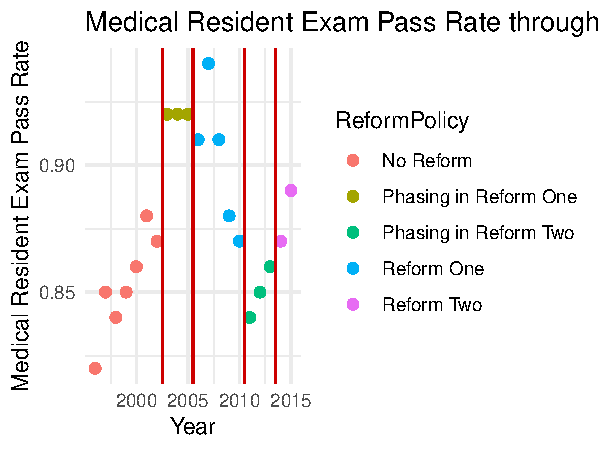
\includegraphics{Report_files/figure-pdf/unnamed-chunk-6-1.pdf}

The plot shown above displays the medical resident exam pass rate over
the years 1996 to 2015. The plot was further split into five sections.
The initial three time periods - no reform policy, reform policy one,
and reform policy two - were further broken down into additional time
periods. Each reform policy was split into a phasing-in time period a
reform policy time period. The phasing-in time period contains the three
years in which students taking the exam took some combination of the
previous reform policy and the new reform policy during their three-year
medical residency.

Students that fall in the section ``Phasing in Reform One'' (green dots
on the plot), had experienced both no reform policy and reform policy
one. Students that fall in the section ``Phasing in Reform Two'' (teal
dots on the plot), had experienced both reform policy one and reform
policy two during their residency.

As can be seen from the plot, students that took the examination in
years where they experienced some amount of reform policy one appeared
to perform better than students that took the examination in years where
they experience no reform policy or some amount of reform policy two.

\section{Model Implementation
Details}\label{model-implementation-details}

\subsubsection{Model 1 - Binomial
Mixture}\label{model-1---binomial-mixture}

We reasonably assumed that exam pass rates contain unobserved
year-to-year variation, such as differences in exam difficulty or cohort
quality. To capture this extra source of randomness, we fit a binomial
mixture model by including a random intercept for each year. This
approach allowed us to separate systematic effects of reform policies
from idiosyncratic annual noise.

We fit a generalized linear mixed model (GLMM) with a logit link,
specifying pass/fail outcomes as the response and reform time period as
the fixed effect, with year as a random effect:

\[
\text{Pass}_{iy} \sim \text{Binomial}(n_{iy}, p_{iy}), \quad \text{logit}(p_{iy}) = \alpha + \beta \cdot \text{timeperiod}_{iy} + u_y, \quad u_y \sim N(0, \sigma^2).
\]

\subsubsection{Model 2 - Beta-binomial}\label{model-2---beta-binomial}

The binomial assumption may underestimate variability in exam outcomes
because pass probabilities likely vary within each period. To allow for
overdispersion, we modeled the yearly pass probabilities as
Beta-distributed. This yields a hierarchical structure where exam
outcomes are drawn from a binomial conditional on the latent
Beta-distributed rate.

We fit a beta-binomial regression with time period as the predictor
using the glmmTMB package with a logit link. The model structure was: \[
\pi_y \sim \text{Beta}(\alpha, \beta), \quad \text{Pass}_y \sim \text{Binomial}(n_y, \pi_y).
\] Here, dispersion was estimated directly from the data, capturing
unmodeled heterogeneity.

\subsubsection{Model 3 - Beta-binomial on
subset}\label{model-3---beta-binomial-on-subset}

Because policy reforms were phased in gradually, exam cohorts in
transition years likely had mixed exposure. To avoid contamination, we
fit the beta-binomial model on a restricted dataset excluding these
phase-in years. This design isolates the effect of reforms once they
were fully implemented.

We restricted the dataset to years 1996--2002, 2006--2010, and
2014--2015. The same beta-binomial specification was used, with time
period as the predictor and a logit link for the mean pass probability.

\section{Model Evaluation}\label{model-evaluation}

To check goodness of fit, we plotted Pearson residuals over time. We
appear to minimize residuals over time in the mixture model, as seen
below. Putting this together, we concluded that the full beta-binomial
mixture model is the best fit.

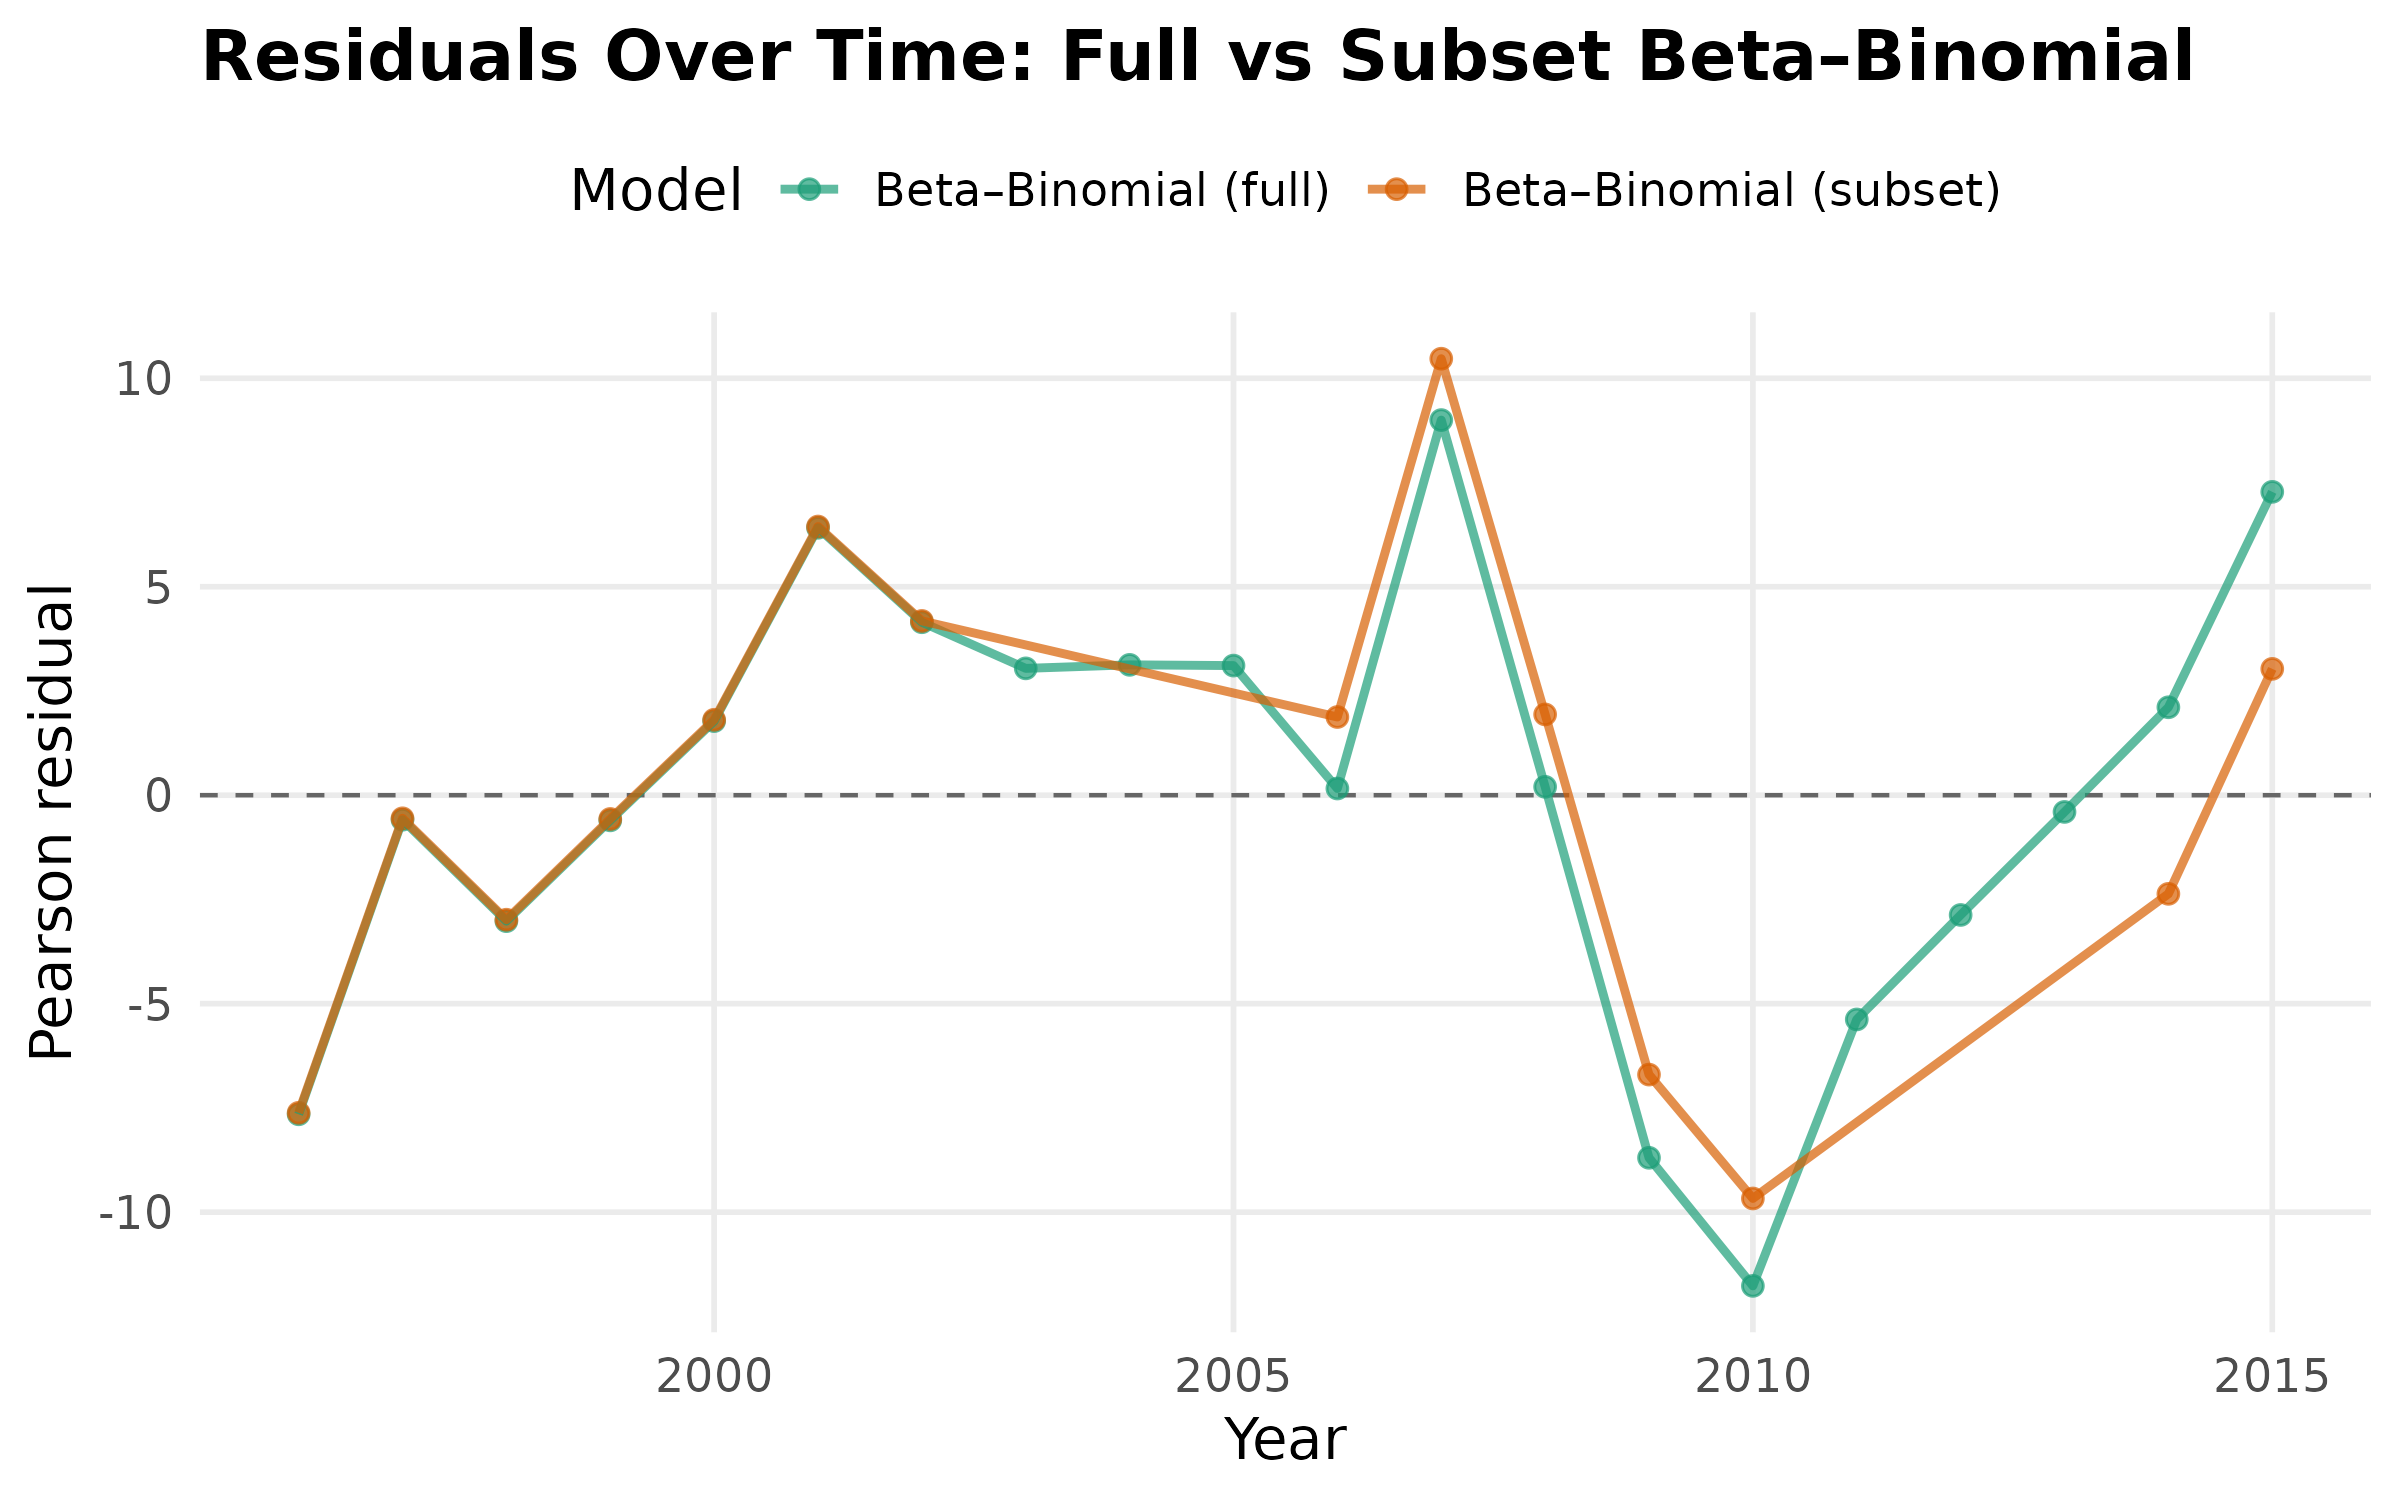
\includegraphics[width=0.8\textwidth,height=\textheight]{residuals_full_vs_subset.png}

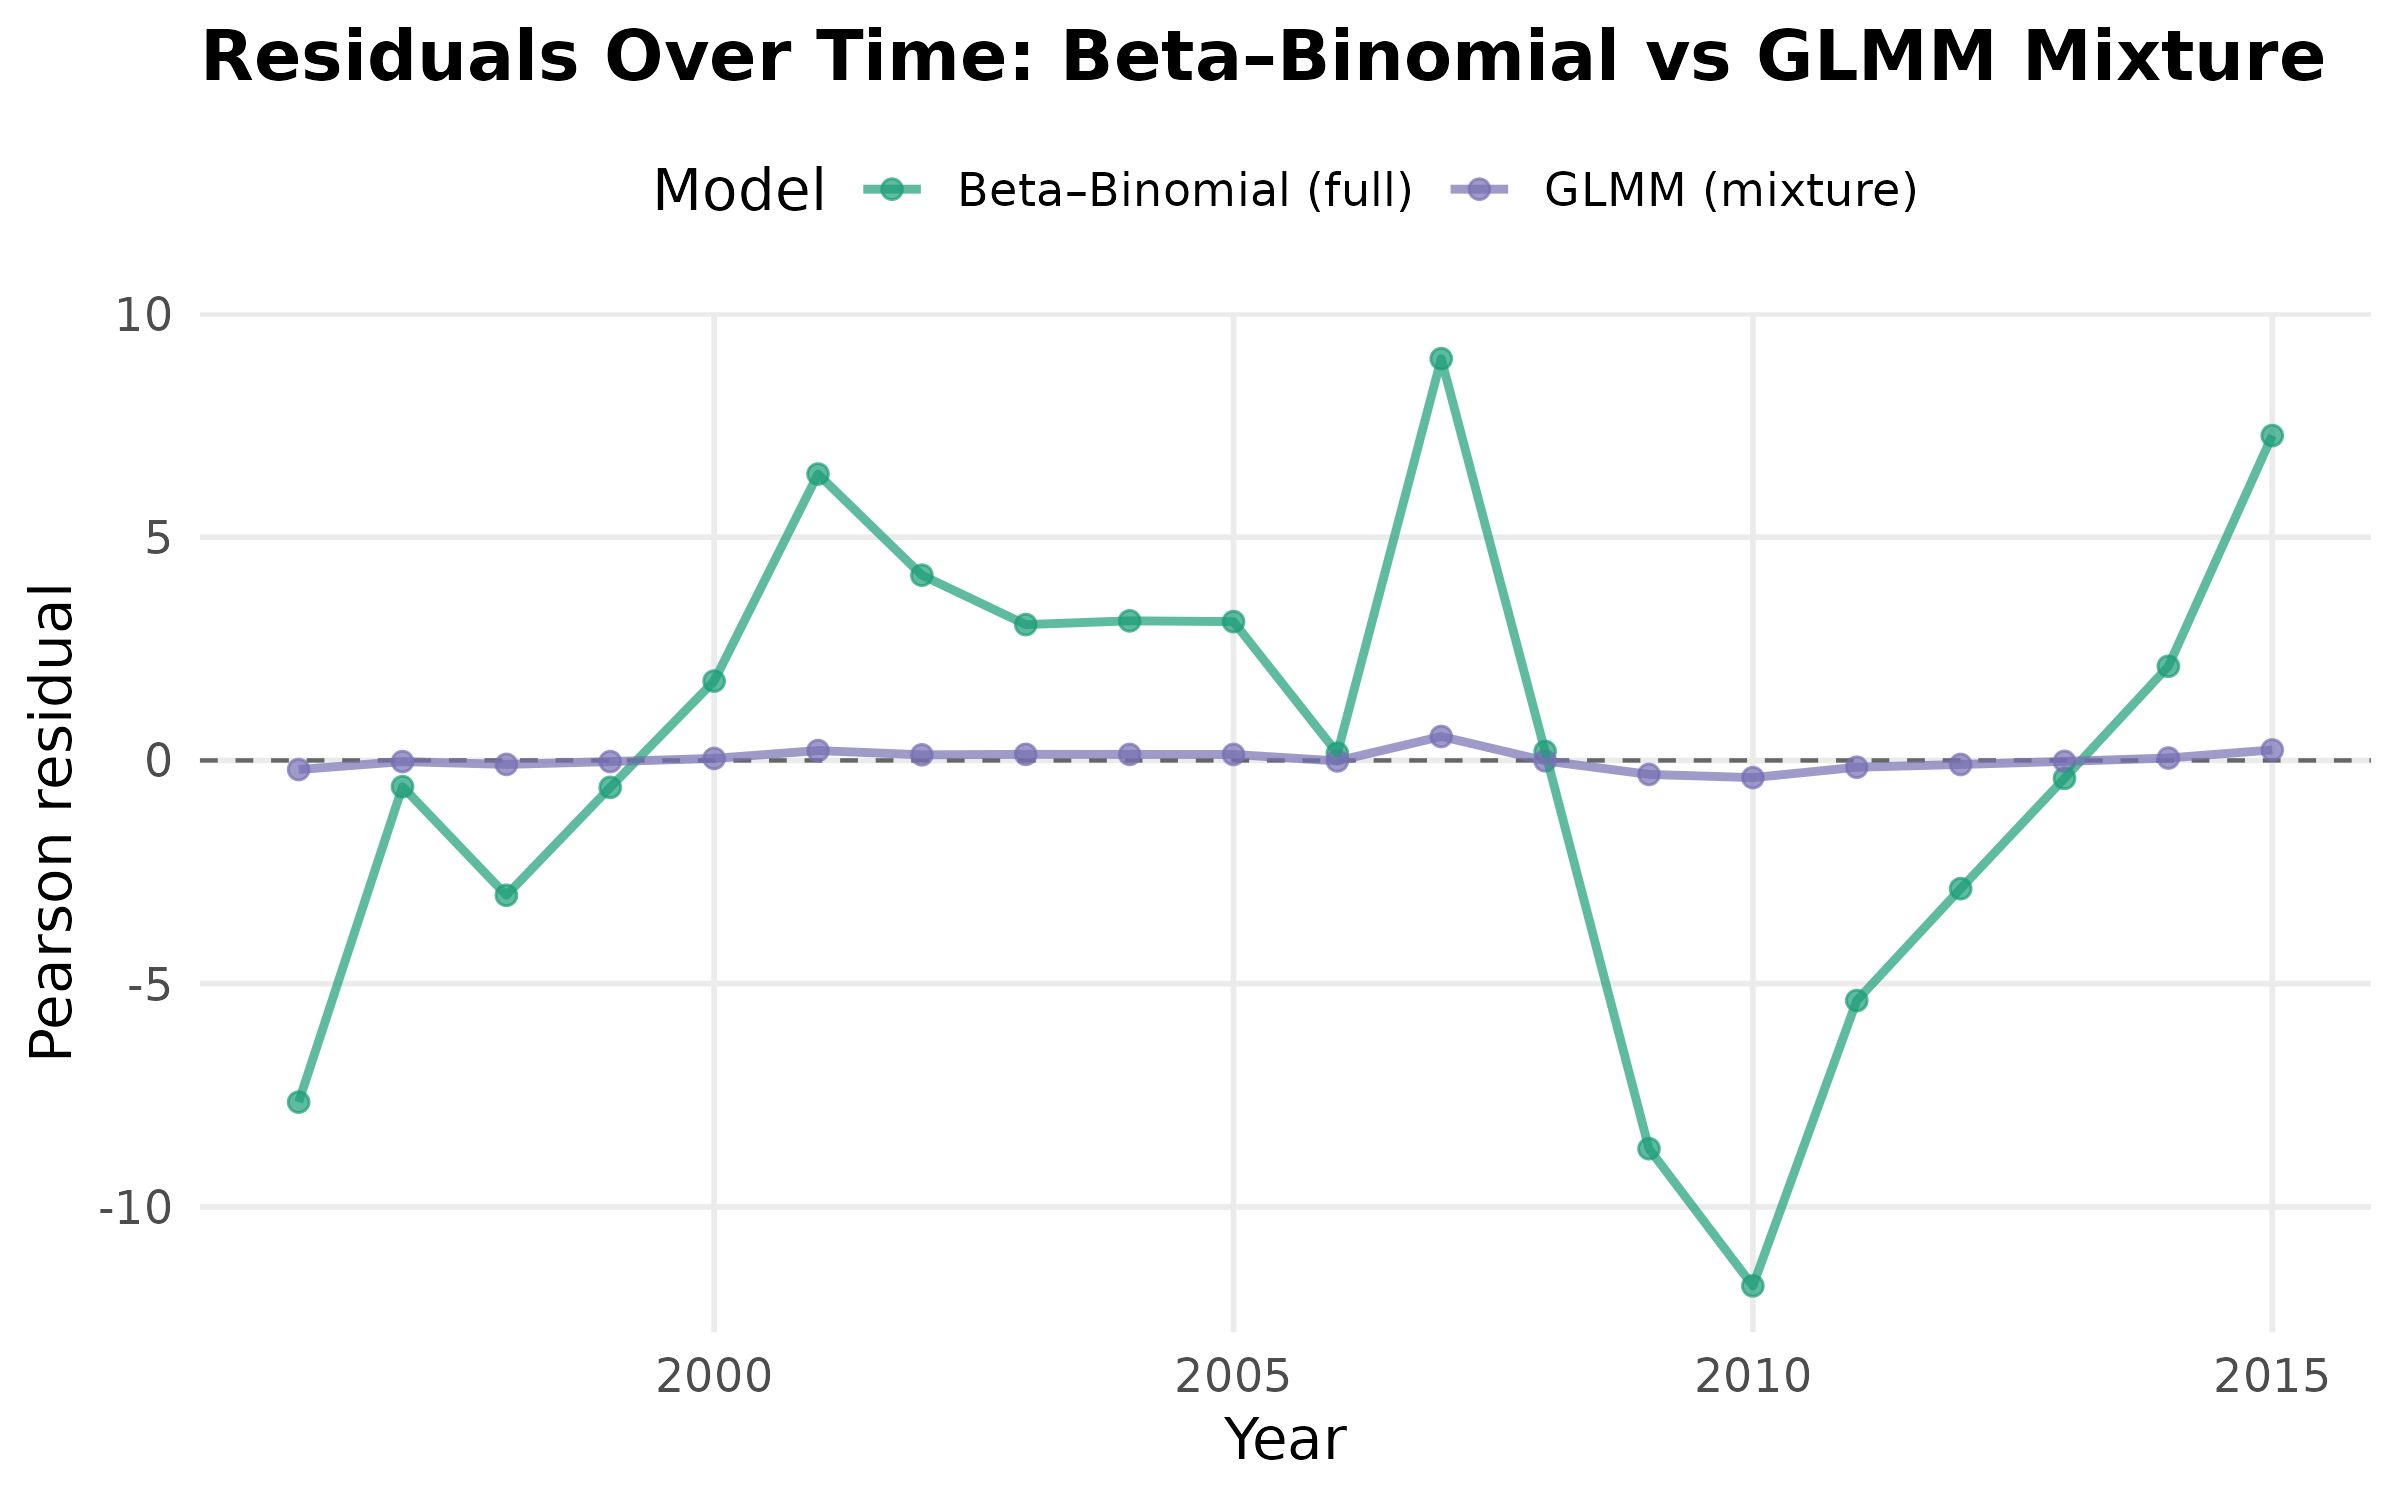
\includegraphics[width=0.8\textwidth,height=\textheight]{residuals_full_vs_mixture.png}

\section{Shortcomings}\label{shortcomings}

An issue came with finding good evaluation metrics that compare across
models. We initially attempted AIC across all models, but soon learned
this was not comparable for any of the models because the mixture
modeling package and beta binomial packages use different formulations
of AIC. In addition, AIC is dependent on the likelihood and because of
this comparing AIC across a full or subset model since they utilize
variable number of observations.

Looking ahead, a next step would be to use Bayesian models, which would
allow us to incorporate auxiliary information into the analysis.

\section{Conclusion}\label{conclusion}

\begin{verbatim}
                Estimate Std. Error   z value      Pr(>|z|)
(Intercept)    2.3234138 0.06885337 33.744374 1.292817e-249
timeperiodtp1 -0.5591105 0.10041764 -5.567851  2.579000e-08
timeperiodtp3 -0.4831369 0.11034058 -4.378597  1.194459e-05
\end{verbatim}

We concluded that the binomial mixture model is the best fit. With that
model, we found that the first reform increased the odds of passing,
while the second reform was associated with a decline in performance.
Both of these were confirmed by significant coefficients.

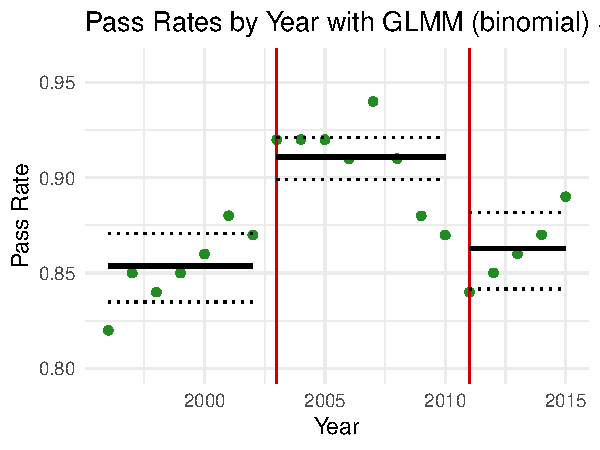
\includegraphics{Report_files/figure-pdf/unnamed-chunk-13-1.pdf}

\section{Citations}\label{citations}

https://www.bmj.com/content/366/bmj.l4134\#:\textasciitilde:text=The\%20first\%20reform\%2C\%20in\%202003,the\%20period\%20of\%20these\%20reforms.
https://jamanetwork.com/journals/jamainternalmedicine/fullarticle/1672284




\end{document}
